\documentclass{beamer}

\usepackage{graphicx}
\usepackage{graphicx}
\usepackage{pgffor}
\usepackage{hyperref}



\setbeamertemplate{navigation symbols}{}
\usetheme{Montpellier}


\begin{document}

\author{by Eszter Domokos-Kővári  \\  \tiny   - based on definintions of Wikipedia -}
	
\title{Nine-point circle} 

\setlength{\parindent}{1em}



    \begin{frame}
    \maketitle
    \end{frame}



    \begin{frame}

	\frametitle{The nine points}

	\begin{figure}

		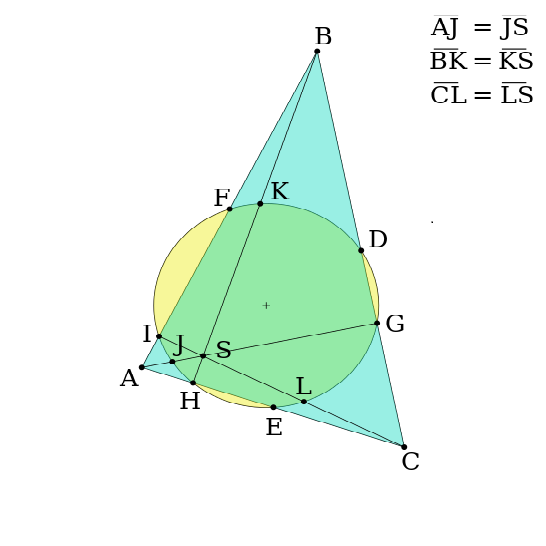
\includegraphics[angle=40, width=9cm]{9points.png}

	\end{figure}

    	\vspace{2 cm}

    \end{frame}

\section{Intro}

\subsection{Denomination}
    \begin{frame}
    	\frametitle{How to define Euler's circle?}
 

     Also known as Feuerbach's circle or Euler's circle
(not to be confused with Euler’s circle in graph theory)
the nine-point circle  (not to be confused with Pont Neuf ;))   \par  

    In geometry, the nine-point circle is a circle
that can be constructed for any given triangle. \par

    It is so named because it passes through
nine significant concyclic points defined from the triangle.


    \end{frame}

\subsection{Definition}

	\begin{frame}

 These nine points are:

    		\begin{itemize}
        		\item The midpoint of each side of the triangle
        		\pause
        		\item The foot of each altitude
        		\pause
        		\item The midpoint of the line segment from each vertex of the triangle to the orthocenter
        (where the three altitudes meet; these line segments lie on their respective altitudes)     
    		\end{itemize}


	\end{frame}


	\begin{frame}
    		\begin{itemize}
        		\item The midpoint of each side of the triangle \cite{2}
       
        		\item The foot of each altitude \cite{3}

        		\item The midpoint of the line segment from each vertex of the triangle to the orthocenter
    		\end{itemize}

		\begin{center}
		    \begin{columns}
		        \begin{column}{3.5cm}
		            \begin{block}{D-F}
		                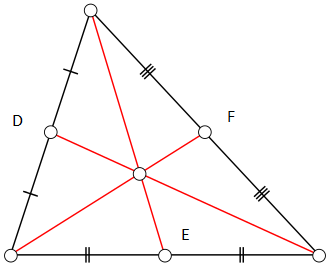
\includegraphics[angle=2.5, width=4cm]{median.png}
		            \end{block}
		        \end{column}
		        \pause
		        \begin{column}{3.5cm}
		            \begin{block}{G-I}
		                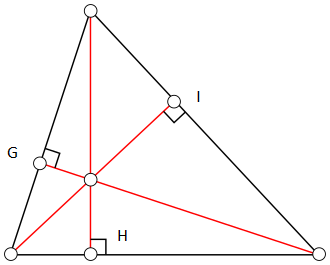
\includegraphics[angle=2.5, width=4cm]{altitudes.png}
		            \end{block}
		        \end{column}
		        \pause
		        \begin{column}{3.5cm}
		            \begin{block}{J-L}
		                \includegraphics[angle=2.5, width=4cm]{medialpoints.png}
		            \end{block}
		        \end{column}
		    \end{columns}
		\end{center}   
	
	    
    
	\end{frame}


	\begin{frame}
	    \begin{itemize}
	        \item The midpoint of each side of the triangle
	
	        \item The foot of each altitude
	
	        \item The midpoint of the line segment from each vertex of the triangle to the orthocenter
	        (where the three altitudes meet; these line segments lie on their respective altitudes) 
	
	   
	    
	    \end{itemize}

   		 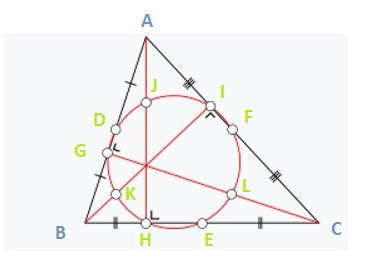
\includegraphics[ width=7cm]{ninepoints.jpg};

	\end{frame}



	\begin{frame}
	
	    \frametitle{Nine significant points}
	 
	        The diagram above shows the nine significant points of the nine-point circle.\\*
		\medskip
	Points D, E, and F are the midpoints of the three sides of the triangle. Points G, H, and I are the feet of the altitudes of the triangle. Points J, K, and L are the midpoints of the line segments between each altitude's vertex intersection (points A, B, and C) and the triangle's orthocenter (point S).
	For an acute triangle, six of the points (the midpoints and altitude feet) lie on the triangle itself; for an obtuse triangle two of the altitudes have feet outside the triangle, but these feet still belong to the nine-point circle.
	\end{frame}
	
	
\section{Animation}
	
	
			\foreach \index in {1, ..., 12} 
			{
			\begin{frame}
		    	\begin{center}
		  	\includegraphics[width=\textwidth]{3szog\index.png}\par%
			\end{center}
			\end{frame}
	  		}


\section{"Extro"}

\subsection{History}

	\begin{frame}


        	\frametitle {Discovery}
    Although he is credited for its discovery, Karl Wilhelm Feuerbach did not entirely discover the nine-point circle, but rather the six-point circle,\\* recognizing the significance of the midpoints of the three sides of the triangle and the feet of the altitudes of that triangle.\par 
		\medskip 
  (At a slightly earlier date, Charles Brianchon and Jean-Victor Poncelet had stated and proven the same theorem.) \par  

	\end{frame}

	\begin{frame}

Soon after Feuerbach, mathematician Olry Terquem himself proved the existence of the circle. \\
	\medskip
He was the first to recognize the added significance of the three midpoints \\
 between the triangle's vertices and the orthocenter. \\*
	\medskip
 Thus, Terquem was the first to use the name nine-point circle. 

	\end{frame}

\subsection{Extras}

	\begin{frame} 

        	\frametitle {Some further properties of the nine-point circle}
    

	 \begin{columns}
           	\begin{column}{0.5cm}
           	\end{column}
           	\begin{column}{9cm}

   			\uncover<1-> {The radius of a triangle's circumcircle is twice the radius of that triangle's nine-point circle.} \par  
    \vspace{0.2cm}
     			\uncover<3-> {A nine-point circle bisects a line segment going from the corresponding triangle's orthocenter to any point on its circumcircle.}
       
    \vspace{0.2cm}

    			\uncover<5-> {The center N of the nine-point circle bisects a segment from the orthocenter H to the circumcenter O
				 (making the orthocenter a center of dilation to both circles)  ON = NH.} \par  

     			\uncover<6> {The nine-point center N is one-fourth of the way along the Euler line from the centroid G to the orthocenter
   					 HN = 3NG.}
	

           	\end{column}

           	\begin{column}{3.5cm}

    			\uncover<2> {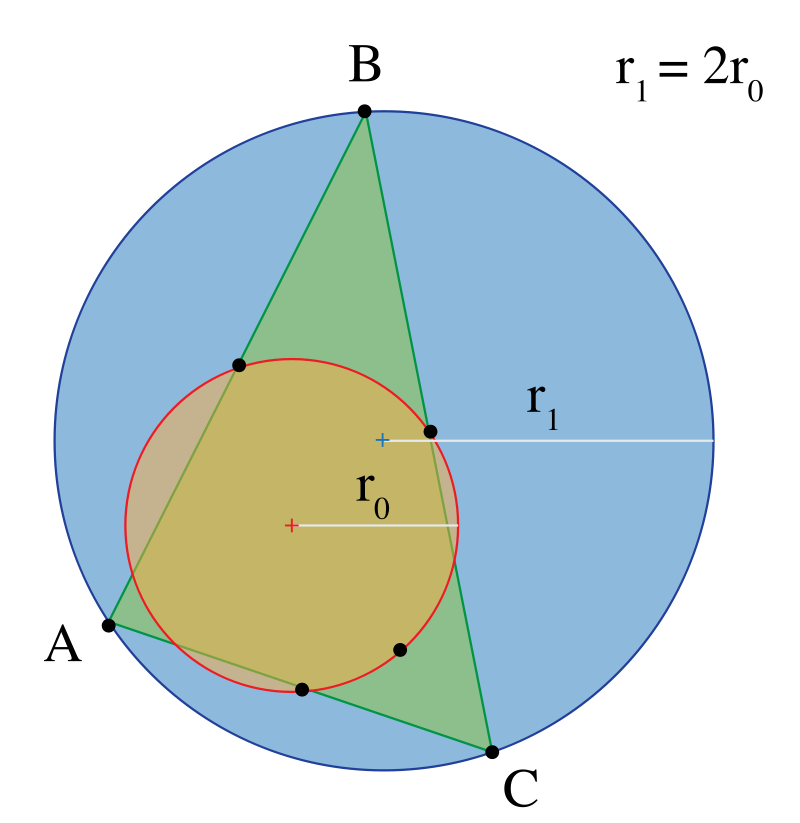
\includegraphics[angle=5, width=3cm]{prop1.png}}

     			\uncover<4> {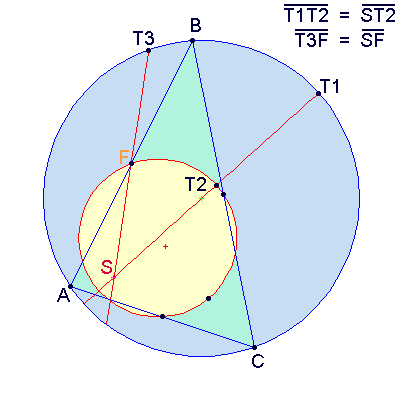
\includegraphics[angle=5, width=3cm]{prop2.png}}

   

           \end{column}
       
\end{columns}




	\end{frame}

\subsection{References}

	\begin{frame}
        	\frametitle{Források}
    			\begin{itemize}
        		\item geogebra
			\item wikipedia

     			\end{itemize}
	\end{frame}




\end{document}